\documentclass[conference]{IEEEtran}
\usepackage{amsmath,amssymb}
\usepackage[T1]{fontenc}
\usepackage{booktabs}
\usepackage{graphicx}
\usepackage{enumitem}
% Author punctuation preference; IEEEtran layout and class remain unchanged.
\usepackage{etoolbox}
\patchcmd{\abstract}{---}{- }{}{\PackageError{paper}{Abstract punctuation patch failed}{}}
\patchcmd{\IEEEkeywords}{---}{- }{}{\PackageError{paper}{Keywords punctuation patch failed}{}}
\usepackage[hidelinks]{hyperref}
\hypersetup{pdftitle={Matching the Wrong Thing: Goal-Frame Velocity in the Planning Cost of a JEPA World Model},
  pdfauthor={Le Van Manh}, pdfkeywords={world models, JEPA, planning, goal-conditioned planning, cost design}}
% Auto-generated by make_numbers_r8.py from JSON outputs. Do not edit by hand.
\newcommand{\DevN}{26}
\newcommand{\DevOff}{3.845}
\newcommand{\DevOffSucc}{7}
\newcommand{\DevOffAgent}{62.3}
\newcommand{\DevOffBlock}{22.9}
\newcommand{\DevOffAngle}{24.2}
\newcommand{\DevEOff}{3.540}
\newcommand{\DevEOffSucc}{6}
\newcommand{\DevEOffAgent}{58.2}
\newcommand{\DevEOffBlock}{19.7}
\newcommand{\DevEOffAngle}{20.6}
\newcommand{\DevPropPred}{3.315}
\newcommand{\DevPropPredSucc}{1}
\newcommand{\DevPropPredAgent}{46.6}
\newcommand{\DevPropPredBlock}{33.4}
\newcommand{\DevPropPredAngle}{27.0}
\newcommand{\DevPropTrue}{3.331}
\newcommand{\DevPropTrueSucc}{1}
\newcommand{\DevPropTrueAgent}{46.6}
\newcommand{\DevPropTrueBlock}{33.8}
\newcommand{\DevPropTrueAngle}{26.9}
\newcommand{\DevAgentOr}{2.971}
\newcommand{\DevAgentOrSucc}{7}
\newcommand{\DevAgentOrAgent}{29.5}
\newcommand{\DevAgentOrBlock}{37.0}
\newcommand{\DevAgentOrAngle}{27.4}
\newcommand{\DevABOr}{2.610}
\newcommand{\DevABOrSucc}{11}
\newcommand{\DevABOrAgent}{37.3}
\newcommand{\DevABOrBlock}{21.8}
\newcommand{\DevABOrAngle}{22.2}
\newcommand{\DevOracle}{2.527}
\newcommand{\DevOracleSucc}{11}
\newcommand{\DevOracleAgent}{40.1}
\newcommand{\DevOracleBlock}{20.9}
\newcommand{\DevOracleAngle}{20.6}
\newcommand{\DevHstd}{3.316}
\newcommand{\DevHstdSucc}{6}
\newcommand{\DevHstdAgent}{51.9}
\newcommand{\DevHstdBlock}{23.0}
\newcommand{\DevHstdAngle}{22.7}
\newcommand{\DevVZ}{3.183}
\newcommand{\DevVZSucc}{10}
\newcommand{\DevVZAgent}{47.0}
\newcommand{\DevVZBlock}{21.7}
\newcommand{\DevVZAngle}{23.5}
\newcommand{\DevVOne}{3.810}
\newcommand{\DevVOneSucc}{6}
\newcommand{\DevVOneAgent}{62.7}
\newcommand{\DevVOneBlock}{21.5}
\newcommand{\DevVOneAngle}{22.9}
\newcommand{\DevPosOnly}{2.936}
\newcommand{\DevPosOnlySucc}{8}
\newcommand{\DevPosOnlyAgent}{32.0}
\newcommand{\DevPosOnlyBlock}{37.4}
\newcommand{\DevPosOnlyAngle}{27.1}
\newcommand{\DevVelOnly}{4.249}
\newcommand{\DevVelOnlySucc}{1}
\newcommand{\DevVelOnlyAgent}{70.5}
\newcommand{\DevVelOnlyBlock}{29.8}
\newcommand{\DevVelOnlyAngle}{26.8}
\newcommand{\DevVzero}{3.275}
\newcommand{\DevVzeroSucc}{7}
\newcommand{\DevVzeroAgent}{50.0}
\newcommand{\DevVzeroBlock}{23.2}
\newcommand{\DevVzeroAngle}{22.9}
\newcommand{\DevVZD}{\ensuremath{-}0.663}
\newcommand{\DevVZImp}{16}
\newcommand{\DevVZWor}{2}
\newcommand{\DevVZDexcl}{\ensuremath{-}0.569}
\newcommand{\DevSharePos}{0.40}
\newcommand{\DevShareVel}{0.73}
\newcommand{\DevShareCross}{\ensuremath{-}0.13}
\newcommand{\DevVarRatio}{0.12}
\newcommand{\DevCorrPosProp}{0.42}
\newcommand{\DevSpProp}{0.40}
\newcommand{\DevSpPos}{0.956}
\newcommand{\DevSpVel}{\ensuremath{-}0.01}
\newcommand{\DevSpPredTrue}{0.996}
\newcommand{\DevResid}{0.019}
\newcommand{\DevGoalSpeed}{79}
\newcommand{\DevCond}{1.86}
\newcommand{\DevBanksWithSucc}{11}
\newcommand{\DevVZHits}{10}
\newcommand{\DevOffHits}{7}
\newcommand{\DevSensMinMean}{2.881}
\newcommand{\DevSensMaxMean}{3.183}
\newcommand{\REightN}{16}
\newcommand{\REightBzero}{2.947}
\newcommand{\REightBzeroLo}{1.707}
\newcommand{\REightBzeroHi}{4.286}
\newcommand{\REightBzeroSucc}{8}
\newcommand{\REightBzeroSp}{0.551}
\newcommand{\REightBone}{2.909}
\newcommand{\REightBoneLo}{1.752}
\newcommand{\REightBoneHi}{4.160}
\newcommand{\REightBoneSucc}{6}
\newcommand{\REightBoneSp}{0.701}
\newcommand{\REightVZ}{2.320}
\newcommand{\REightVZLo}{1.360}
\newcommand{\REightVZHi}{3.339}
\newcommand{\REightVZSucc}{9}
\newcommand{\REightVZSp}{0.794}
\newcommand{\REightHten}{2.722}
\newcommand{\REightHtenLo}{1.705}
\newcommand{\REightHtenHi}{3.792}
\newcommand{\REightHtenSucc}{5}
\newcommand{\REightHtenSp}{0.569}
\newcommand{\REightHstd}{2.918}
\newcommand{\REightHstdLo}{1.802}
\newcommand{\REightHstdHi}{4.147}
\newcommand{\REightHstdSucc}{4}
\newcommand{\REightHstdSp}{0.596}
\newcommand{\REightTpe}{2.708}
\newcommand{\REightTpeLo}{1.526}
\newcommand{\REightTpeHi}{3.973}
\newcommand{\REightTpeSucc}{8}
\newcommand{\REightTpeSp}{0.642}
\newcommand{\REightPow}{2.486}
\newcommand{\REightPowLo}{1.404}
\newcommand{\REightPowHi}{3.665}
\newcommand{\REightPowSucc}{9}
\newcommand{\REightPowSp}{0.645}
\newcommand{\REightFix}{3.190}
\newcommand{\REightFixLo}{1.816}
\newcommand{\REightFixHi}{4.647}
\newcommand{\REightFixSucc}{8}
\newcommand{\REightFixSp}{0.573}
\newcommand{\REightPosOnly}{2.584}
\newcommand{\REightPosOnlyLo}{1.533}
\newcommand{\REightPosOnlyHi}{3.712}
\newcommand{\REightPosOnlySucc}{7}
\newcommand{\REightPosOnlySp}{0.863}
\newcommand{\REightVOne}{2.946}
\newcommand{\REightVOneLo}{1.707}
\newcommand{\REightVOneHi}{4.285}
\newcommand{\REightVOneSucc}{8}
\newcommand{\REightVOneSp}{0.552}
\newcommand{\REightEBzero}{2.838}
\newcommand{\REightEBzeroLo}{1.554}
\newcommand{\REightEBzeroHi}{4.243}
\newcommand{\REightEBzeroSucc}{7}
\newcommand{\REightEBzeroSp}{0.530}
\newcommand{\REightEBone}{2.654}
\newcommand{\REightEBoneLo}{1.569}
\newcommand{\REightEBoneHi}{3.798}
\newcommand{\REightEBoneSucc}{7}
\newcommand{\REightEBoneSp}{0.721}
\newcommand{\REightOracle}{1.966}
\newcommand{\REightOracleSucc}{9}
\newcommand{\REightRandom}{4.183}
\newcommand{\REightVZDecision}{SUPPORTED}
\newcommand{\REightVZD}{\ensuremath{-}0.627}
\newcommand{\REightVZDLo}{\ensuremath{-}1.298}
\newcommand{\REightVZDHi}{\ensuremath{-}0.110}
\newcommand{\REightVZImp}{7}
\newcommand{\REightVZWor}{1}
\newcommand{\REightVZDexcl}{\ensuremath{-}0.371}
\newcommand{\REightVZGain}{1}
\newcommand{\REightVZLoss}{0}
\newcommand{\REightBoneDecision}{NOT\_REPLICATED}
\newcommand{\REightBoneD}{\ensuremath{-}0.038}
\newcommand{\REightBoneDLo}{\ensuremath{-}0.612}
\newcommand{\REightBoneDHi}{0.530}
\newcommand{\REightBoneImp}{7}
\newcommand{\REightBoneWor}{7}
\newcommand{\REightBoneDexcl}{0.143}
\newcommand{\REightMechDecision}{REPLICATED}
\newcommand{\REightSpProp}{0.43}
\newcommand{\REightSpPos}{0.954}
\newcommand{\REightShareVel}{0.64}
\newcommand{\REightVZminusBone}{\ensuremath{-}0.589}
\newcommand{\REightVZminusBoneLo}{\ensuremath{-}1.207}
\newcommand{\REightVZminusBoneHi}{\ensuremath{-}0.047}
\newcommand{\REightVZvsBoneGain}{3}
\newcommand{\REightVZvsBoneLoss}{0}
\newcommand{\RSevenTpeD}{\ensuremath{-}0.053}
\newcommand{\RSevenTpeDLo}{\ensuremath{-}0.826}
\newcommand{\RSevenTpeDHi}{0.797}
\newcommand{\RSevenTpeImp}{4}
\newcommand{\RSevenTpeWor}{4}
\newcommand{\RSevenProbeN}{1267}
\newcommand{\RSevenOffSp}{0.795}
\newcommand{\RSevenPaeSp}{0.754}
\newcommand{\RSevenOffRot}{0.853}
\newcommand{\RNineN}{16}
\newcommand{\RNineVZDecision}{SUPPORTED}
\newcommand{\RNineVZD}{\ensuremath{-}1.468}
\newcommand{\RNineVZDLo}{\ensuremath{-}2.814}
\newcommand{\RNineVZDHi}{\ensuremath{-}0.296}
\newcommand{\RNineVZImp}{13}
\newcommand{\RNineVZWor}{3}
\newcommand{\RNineVZDexcl}{\ensuremath{-}1.042}
\newcommand{\RNineVZGain}{5}
\newcommand{\RNineVZLoss}{1}
\newcommand{\RNineBoneDecision}{NO\_SIGNAL}
\newcommand{\RNineBoneD}{2.343}
\newcommand{\RNineBoneDLo}{\ensuremath{-}0.078}
\newcommand{\RNineBoneDHi}{5.335}
\newcommand{\RNineBoneImp}{6}
\newcommand{\RNineBoneWor}{10}
\newcommand{\RNineBoneDexcl}{2.830}
\newcommand{\RNineBoneGain}{0}
\newcommand{\RNineBoneLoss}{4}
\newcommand{\RNineBzeroMargin}{3.059}
\newcommand{\RNineBzeroSucc}{7}
\newcommand{\RNineBzeroBlockOnly}{12}
\newcommand{\RNineVZMargin}{1.591}
\newcommand{\RNineVZSucc}{11}
\newcommand{\RNineVZBlockOnly}{12}
\newcommand{\RNineBoneMargin}{5.402}
\newcommand{\RNineBoneSucc}{3}
\newcommand{\RNineBoneBlockOnly}{4}
\newcommand{\RNineVZminusBone}{\ensuremath{-}3.811}
\newcommand{\RNineVZminusBoneLo}{\ensuremath{-}6.428}
\newcommand{\RNineVZminusBoneHi}{\ensuremath{-}1.666}
\newcommand{\RNineBzeroAgent}{49.3}
\newcommand{\RNineBzeroBlock}{26.1}
\newcommand{\RNineBzeroAngle}{16.6}
\newcommand{\RNineBzeroMarginLo}{1.698}
\newcommand{\RNineBzeroMarginHi}{4.476}
\newcommand{\RNineVZAgent}{16.8}
\newcommand{\RNineVZBlock}{22.9}
\newcommand{\RNineVZAngle}{10.8}
\newcommand{\RNineVZMarginLo}{0.817}
\newcommand{\RNineVZMarginHi}{2.536}
\newcommand{\RNineBoneAgent}{83.7}
\newcommand{\RNineBoneBlock}{51.0}
\newcommand{\RNineBoneAngle}{25.5}
\newcommand{\RNineBoneMarginLo}{3.058}
\newcommand{\RNineBoneMarginHi}{8.228}
\newcommand{\RNineEliteRawVZ}{0.287}
\newcommand{\RNineEliteRawBone}{0.551}
\newcommand{\RNineFracNegBone}{0.9}
\newcommand{\OptRawVZ}{0.94}
\newcommand{\OptBoneVZ}{1.01}
\newcommand{\OptPosVZ}{0.75}
\newcommand{\OptRawBone}{1.11}
\newcommand{\OptBoneBone}{1.08}
\newcommand{\OptPosBone}{1.08}
\newcommand{\OptRawBzero}{1.05}
\newcommand{\OptBoneBzero}{1.08}
\newcommand{\OptPosBzero}{1.02}
\newcommand{\RTenN}{8}
\newcommand{\RTenVZDecision}{SUPPORTED}
\newcommand{\RTenVZD}{\ensuremath{-}0.355}
\newcommand{\RTenVZDLo}{\ensuremath{-}0.822}
\newcommand{\RTenVZDHi}{\ensuremath{-}0.051}
\newcommand{\RTenVZImp}{3}
\newcommand{\RTenVZWor}{0}
\newcommand{\RTenVZDexcl}{\ensuremath{-}0.139}
\newcommand{\RTenBzero}{3.862}
\newcommand{\RTenBzeroSucc}{2}
\newcommand{\RTenVZ}{3.506}
\newcommand{\RTenVZSucc}{2}
\newcommand{\RTenHstd}{3.506}
\newcommand{\RTenHstdSucc}{2}
\newcommand{\RTenHten}{3.159}
\newcommand{\RTenHtenSucc}{2}
\newcommand{\RTenBone}{3.709}
\newcommand{\RTenBoneSucc}{2}
\newcommand{\RTenOracle}{3.060}
\newcommand{\RTenOracleSucc}{2}
\newcommand{\RTenMechDecision}{NOT\_REPLICATED}
\newcommand{\RTenSpProp}{0.98}
\newcommand{\RTenSpPos}{0.968}
\newcommand{\RTenShareVel}{0.015}
\newcommand{\RTenDexcl}{\ensuremath{-}0.139}
\newcommand{\RTenUnchanged}{5}
\newcommand{\RTenPosOnly}{3.116}
\newcommand{\RTenVOne}{3.862}
\newcommand{\RTenRandom}{4.999}
\newcommand{\RTenBoneD}{\ensuremath{-}0.152}
\newcommand{\EncJepaRatio}{0.85}
\newcommand{\EncDinoRatio}{0.025}
\newcommand{\EncDinoVx}{0.021}
\newcommand{\EncDinoVy}{0.019}
\newcommand{\EncDinoX}{0.88}
\newcommand{\EncDinoY}{0.73}
\newcommand{\EncJepaVx}{0.61}
\newcommand{\EncJepaVy}{0.57}
\newcommand{\EncJepaX}{0.80}
\newcommand{\EncJepaY}{0.57}
\newcommand{\SameSelJepa}{2}
\newcommand{\SameSelJepaN}{16}
\newcommand{\SameSelDino}{8}
\newcommand{\SameSelDinoN}{8}

% Copied verbatim from the auto-generated numbers block of R6_WORKING_DRAFT.tex (make_numbers.py, R6 package, 26/10/2026).
% Only the macros cited in the R8 draft are kept; values unchanged.
\newcommand{\RsixNtest}{10}
\newcommand{\RsixNtrain}{16}
\newcommand{\RsixD}{\ensuremath{-}0.758}
\newcommand{\RsixDLo}{\ensuremath{-}1.473}
\newcommand{\RsixDHi}{\ensuremath{-}0.117}
\newcommand{\RsixMarginBzero}{4.363}
\newcommand{\RsixSuccBzero}{2}
\newcommand{\RsixMarginBone}{3.604}
\newcommand{\RsixSuccBone}{4}
\newcommand{\RsixMarginEBzero}{4.238}
\newcommand{\RsixRefOracle}{2.987}
\newcommand{\HpropD}{\ensuremath{-}0.588}
\newcommand{\HpropDLo}{\ensuremath{-}1.167}
\newcommand{\HpropDHi}{0.005}
\newcommand{\HpropSuccOfficial}{2}
\newcommand{\HpropSuccLam}{1}
\newcommand{\RfiveDecision}{FUTILE for this setting}
\newcommand{\RfiveDone}{0.080}
\newcommand{\RfiveDoneLo}{0.000}
\newcommand{\RfiveDoneHi}{0.239}
\newcommand{\DinoDone}{0.000}
\newcommand{\RfiveProbeRidgeMinusBestCal}{0.341}
\newcommand{\PbbNormB}{0.758}
\newcommand{\PbbNormA}{0.970}

% Auto-generated by make_numbers_extra.py. Do not edit by hand.
\newcommand{\DecJPos}{35.5\%}
\newcommand{\DecJVel}{62.7\%}
\newcommand{\DecJCross}{1.6\%}
\newcommand{\DecJResTok}{0.17\%}
\newcommand{\DecJNetRemoved}{64.5\%}
\newcommand{\DecJSpVel}{\ensuremath{-}0.01}
\newcommand{\DecJSpPos}{0.954}
\newcommand{\DecJSpFull}{0.433}
\newcommand{\DecJIdErr}{3\times10^{-15}}
\newcommand{\DecJSpVelMin}{\ensuremath{-}0.307}
\newcommand{\DecJSpVelMax}{0.347}
\newcommand{\DecJVelPooled}{61.0\%}
\newcommand{\DecDnPos}{98.5\%}
\newcommand{\DecDnVel}{0.6\%}
\newcommand{\DecDnCross}{0.9\%}
\newcommand{\DecDnResTok}{0.06\%}
\newcommand{\DecDnNetRemoved}{1.5\%}
\newcommand{\DecDnSpVel}{0.10}
\newcommand{\DecDnSpPos}{0.968}
\newcommand{\DecDnSpFull}{0.980}
\newcommand{\DecDnIdErr}{5\times10^{-15}}
\newcommand{\DecDnSpVelMin}{\ensuremath{-}0.370}
\newcommand{\DecDnSpVelMax}{0.497}
\newcommand{\DecDnVelPooled}{0.4\%}
\newcommand{\CondJ}{2.20}
\newcommand{\AngJ}{59.1}
\newcommand{\GainJ}{1.17}
\newcommand{\CondDn}{2562.2}
\newcommand{\AngDn}{1.0}
\newcommand{\GainDn}{56.64}
\newcommand{\FacRaCzz}{2.947}
\newcommand{\FacRaCzzSucc}{8}
\newcommand{\FacRaCoz}{2.946}
\newcommand{\FacRaCozSucc}{8}
\newcommand{\FacRaCzo}{2.918}
\newcommand{\FacRaCzoSucc}{4}
\newcommand{\FacRaCoo}{2.320}
\newcommand{\FacRaCooSucc}{9}
\newcommand{\FacRaSA}{2.316}
\newcommand{\FacRaSASucc}{9}
\newcommand{\FacRaDropD}{\ensuremath{-}0.598}
\newcommand{\FacRaDropGain}{5}
\newcommand{\FacRaDropLoss}{0}
\newcommand{\FacRaDropMcN}{0.0625}
\newcommand{\FacRtCzz}{3.862}
\newcommand{\FacRtCzzSucc}{2}
\newcommand{\FacRtCoz}{3.862}
\newcommand{\FacRtCozSucc}{2}
\newcommand{\FacRtCzo}{3.506}
\newcommand{\FacRtCzoSucc}{2}
\newcommand{\FacRtCoo}{3.506}
\newcommand{\FacRtCooSucc}{2}
\newcommand{\FacRtSA}{3.506}
\newcommand{\FacRtSASucc}{2}
\newcommand{\FacRtDropD}{0.000}
\newcommand{\FacRtDropGain}{0}
\newcommand{\FacRtDropLoss}{0}
\newcommand{\FacRtDropMcN}{1.0000}
\newcommand{\McNREight}{1.000}
\newcommand{\McNRNine}{0.219}
\newcommand{\SignRNine}{0.0213}
\newcommand{\McNRNineBone}{0.125}
\newcommand{\RNineBoneGainN}{0}
\newcommand{\RNineBoneLossN}{4}
\newcommand{\SignRTen}{0.25}
\newcommand{\BootZeroRTen}{0.0233}
\newcommand{\BoneOwnBone}{0.959}
\newcommand{\BoneOwnBzero}{0.933}
\newcommand{\BoneOwnWorse}{7}
\newcommand{\BoneOwnN}{16}
\newcommand{\RElN}{16}
\newcommand{\RElDecision}{DROP\_HELPS}
\newcommand{\RElD}{\ensuremath{-}0.358}
\newcommand{\RElDLo}{\ensuremath{-}0.790}
\newcommand{\RElDHi}{0.006}
\newcommand{\RElImp}{10}
\newcommand{\RElWor}{6}
\newcommand{\RElUnch}{0}
\newcommand{\RElDexcl}{\ensuremath{-}0.210}
\newcommand{\RElGain}{4}
\newcommand{\RElLoss}{0}
\newcommand{\RElMcN}{0.125}
\newcommand{\RElCzz}{3.059}
\newcommand{\RElCzzSucc}{7}
\newcommand{\RElCzzAgent}{49.3}
\newcommand{\RElCzzBO}{12}
\newcommand{\RElCoz}{2.983}
\newcommand{\RElCozSucc}{7}
\newcommand{\RElCozAgent}{47.4}
\newcommand{\RElCozBO}{11}
\newcommand{\RElCzo}{1.949}
\newcommand{\RElCzoSucc}{7}
\newcommand{\RElCzoAgent}{24.4}
\newcommand{\RElCzoBO}{12}
\newcommand{\RElCoo}{1.591}
\newcommand{\RElCooSucc}{11}
\newcommand{\RElCooAgent}{16.8}
\newcommand{\RElCooBO}{12}
\newcommand{\RElSecD}{\ensuremath{-}0.075}
\newcommand{\RElSecDLo}{\ensuremath{-}0.437}
\newcommand{\RElSecDHi}{0.294}
\newcommand{\RElInter}{\ensuremath{-}0.283}
\newcommand{\RElInterLo}{\ensuremath{-}0.760}
\newcommand{\RElInterHi}{0.181}
\newcommand{\RElScaleFull}{\ensuremath{-}1.110}
\newcommand{\RElScaleFullLo}{\ensuremath{-}2.328}
\newcommand{\RElScaleFullHi}{\ensuremath{-}0.108}
\newcommand{\RElScalePos}{\ensuremath{-}1.393}
\newcommand{\RElMedian}{\ensuremath{-}0.176}
\newcommand{\RElSign}{0.45}
\newcommand{\RElScaleFullGain}{1}
\newcommand{\RElScaleFullLoss}{1}
\newcommand{\RElScaleFullImp}{10}
\newcommand{\RElScaleFullWor}{6}
\newcommand{\RElSecGain}{1}
\newcommand{\RElSecLoss}{1}
\newcommand{\RElCzzBlock}{26.1}
\newcommand{\RElCooBlock}{22.9}
\newcommand{\RElEffFold}{99}
\newcommand{\RElAlphaFull}{9.88}
\newcommand{\RElAlphaPos}{11.34}
\newcommand{\RElVOnePosRatio}{91}
\newcommand{\RElVOnePosRatioMin}{5.8}
\newcommand{\RElAlphaFullMin}{0.247}
\newcommand{\RElAlphaFullMax}{45.636}
\newcommand{\RElNPop}{128}
\newcommand{\FpDnN}{8}
\newcommand{\FpDnChanges}{0}
\newcommand{\FpDnMaxRel}{5.4\%}
\newcommand{\FpDnExact}{yes}
\newcommand{\FpJN}{4}
\newcommand{\FpJChanges}{0}
\newcommand{\FpJMaxRel}{0.4\%}
\newcommand{\FpJExact}{yes}

% Auto-generated by make_numbers_r12.py from r12_analysis.json. Do not edit by hand.
\newcommand{\RTwN}{32}
\newcommand{\RTwRawMargin}{3.057}
\newcommand{\RTwRawSucc}{13}
\newcommand{\RTwRawAgent}{52.9}
\newcommand{\RTwRawBlock}{19.3}
\newcommand{\RTwRawBO}{21}
\newcommand{\RTwFFMargin}{2.597}
\newcommand{\RTwFFSucc}{14}
\newcommand{\RTwFFAgent}{43.9}
\newcommand{\RTwFFBlock}{18.9}
\newcommand{\RTwFFBO}{23}
\newcommand{\RTwFPMargin}{2.429}
\newcommand{\RTwFPSucc}{14}
\newcommand{\RTwFPAgent}{39.9}
\newcommand{\RTwFPBlock}{17.4}
\newcommand{\RTwFPBO}{23}
\newcommand{\RTwVZMargin}{1.562}
\newcommand{\RTwVZSucc}{20}
\newcommand{\RTwVZAgent}{16.5}
\newcommand{\RTwVZBlock}{23.4}
\newcommand{\RTwVZBO}{22}
\newcommand{\RTwQOneDecision}{POSITION\_HELPS}
\newcommand{\RTwQOneD}{\ensuremath{-}0.169}
\newcommand{\RTwQOneLo}{\ensuremath{-}0.430}
\newcommand{\RTwQOneHi}{0.091}
\newcommand{\RTwQOneMed}{\ensuremath{-}0.136}
\newcommand{\RTwQOneImp}{22}
\newcommand{\RTwQOneWor}{10}
\newcommand{\RTwQOneGain}{1}
\newcommand{\RTwQOneLoss}{1}
\newcommand{\RTwQOneMcN}{1.0000}
\newcommand{\RTwQOneSign}{0.0501}
\newcommand{\RTwQOneLBO}{\ensuremath{-}0.087}
\newcommand{\RTwQTwoDecision}{VELDROP\_Z\_HELPS}
\newcommand{\RTwQTwoD}{\ensuremath{-}1.495}
\newcommand{\RTwQTwoLo}{\ensuremath{-}2.445}
\newcommand{\RTwQTwoHi}{\ensuremath{-}0.724}
\newcommand{\RTwQTwoMed}{\ensuremath{-}0.539}
\newcommand{\RTwQTwoImp}{26}
\newcommand{\RTwQTwoWor}{6}
\newcommand{\RTwQTwoGain}{7}
\newcommand{\RTwQTwoLoss}{0}
\newcommand{\RTwQTwoMcN}{0.0156}
\newcommand{\RTwQTwoSign}{0.0005}
\newcommand{\RTwQTwoLBO}{\ensuremath{-}1.189}
\newcommand{\RTwFFRawD}{\ensuremath{-}0.460}
\newcommand{\RTwFFRawLo}{\ensuremath{-}0.857}
\newcommand{\RTwFFRawHi}{\ensuremath{-}0.145}
\newcommand{\RTwFFRawGain}{2}
\newcommand{\RTwFFRawLoss}{1}
\newcommand{\RTwFPRawD}{\ensuremath{-}0.629}
\newcommand{\RTwFPRawLo}{\ensuremath{-}0.991}
\newcommand{\RTwFPRawHi}{\ensuremath{-}0.328}
\newcommand{\RTwFPRawGain}{2}
\newcommand{\RTwFPRawLoss}{1}
\newcommand{\RTwVZFPD}{\ensuremath{-}0.867}
\newcommand{\RTwVZFPLo}{\ensuremath{-}1.590}
\newcommand{\RTwVZFPHi}{\ensuremath{-}0.294}
\newcommand{\RTwVZFPGain}{6}
\newcommand{\RTwVZFPLoss}{0}
\newcommand{\RTwVZFFD}{\ensuremath{-}1.035}
\newcommand{\RTwVZFFLo}{\ensuremath{-}1.721}
\newcommand{\RTwVZFFHi}{\ensuremath{-}0.439}
\newcommand{\RTwVZFFGain}{6}
\newcommand{\RTwVZFFLoss}{0}
\newcommand{\RTwAlphaMean}{1.64}
\newcommand{\RTwAlphaMed}{1.57}
\newcommand{\RTwAlphaMin}{0.34}
\newcommand{\RTwAlphaMax}{4.07}
\newcommand{\RTwAlphaFold}{16}
\newcommand{\RTwVZWFirst}{3.74}
\newcommand{\RTwVZWLast}{23.47}

% Auto-generated by make_numbers_r13.py from r13_analysis.json. Do not edit by hand.
\newcommand{\RThDecision}{DROP\_HELPS\_FRESH}
\newcommand{\RThD}{\ensuremath{-}0.324}
\newcommand{\RThLo}{\ensuremath{-}0.808}
\newcommand{\RThHi}{0.073}
\newcommand{\RThMed}{\ensuremath{-}0.183}
\newcommand{\RThImp}{21}
\newcommand{\RThWor}{11}
\newcommand{\RThGain}{6}
\newcommand{\RThLoss}{0}
\newcommand{\RThMcN}{0.0312}
\newcommand{\RThSign}{0.1102}
\newcommand{\RThLBO}{\ensuremath{-}0.165}
\newcommand{\RThMargin}{1.887}
\newcommand{\RThSucc}{14}
\newcommand{\RThAgent}{23.3}
\newcommand{\RThBlock}{22.1}
\newcommand{\RThBO}{23}
\newcommand{\RThStdRawD}{\ensuremath{-}1.171}
\newcommand{\RThStdRawLo}{\ensuremath{-}2.024}
\newcommand{\RThStdRawHi}{\ensuremath{-}0.520}
\newcommand{\RThStdRawGain}{2}
\newcommand{\RThStdRawLoss}{1}

% Auto-generated by make_numbers_v4.py. Do not edit by hand.
\newcommand{\RaVisOnly}{2.946}
\newcommand{\RaVisOnlySucc}{8}
\newcommand{\RaVisOnlySame}{15}
\newcommand{\RaVisOnlyN}{16}
\newcommand{\DevSensSuccMin}{9}
\newcommand{\DevSensSuccMax}{10}
\newcommand{\DevSensLamMin}{0.75}
\newcommand{\DevSensLamMax}{5}

\newenvironment{widetable}[1][t]{\begin{table*}[#1]}{\end{table*}}
\newcommand{\auditfigwidth}{\columnwidth}

\begin{document}
\title{Matching the Wrong Thing: Goal-Frame Velocity in the Planning Cost of a JEPA World Model}
\author{\IEEEauthorblockN{Le Van Manh}
\IEEEauthorblockA{\textit{Faculty of Information Technology and Communications} \\
\textit{CMC University}\\
Ha Noi, Viet Nam \\
BAI250042@st.cmcu.edu.vn \\
\href{https://github.com/levanmanh268}{github.com/levanmanh268}}}
\maketitle

\begin{abstract}
Goal observations can contain state variables that a task's success criterion does not ask the agent to reproduce. I
examine one such case in the released JEPA-WM planner on PushT: its proprioceptive goal cost penalises the velocity
recorded in the goal frame, although the release's endpoint success criterion ignores velocity. Because the proprioceptive
encoder is linear, this cost decomposes exactly; on the planner's own candidates, velocity accounts for \DecJVel{} of its energy and has a
mean within-bank rank correlation of \DecJSpVel{} with the final agent distance, against \DecJSpPos{} for the position
part. Using the model's own encoder, I construct VELDROP-z, which keeps the decoded position energy and standardises it
against the visual term, without retraining or outcome labels at inference. On a fresh cohort of \RTwN{} starts,
reduced-budget cross-entropy search with VELDROP-z lowered the mean executed margin from \RTwRawMargin{} to
\RTwVZMargin{} (paired difference \RTwQTwoD{} [\RTwQTwoLo, \RTwQTwoHi]) and raised successes from \RTwRawSucc{} to
\RTwVZSucc{} with no losses, repeating an earlier result on \RNineN{} goals. The pre-specified primary comparison,
position against full proprioception at a shared frozen weight, remained uncertain (\RTwQOneD{} [\RTwQOneLo,
\RTwQOneHi]). An exploratory arm added after that analysis standardised the full term; \mbox{VELDROP-z} gained \RThGain{}
successes over it without losses, with an uncertain margin difference (\RThD{} [\RThLo, \RThHi]), and this contrast
also changes the adaptive weight, so it does not isolate a velocity-only effect. The evaluation uses released
checkpoints, training-split goals, a reduced search budget and open-loop execution. The results support a scoped
correction to a released planning cost and identify the evaluations needed before broader claims.

\end{abstract}

\begin{IEEEkeywords}
world models, joint-embedding predictive architecture, open-loop planning, goal-conditioned planning, cost
design, reproducibility
\end{IEEEkeywords}

\section{Introduction}
Goal-conditioned latent world models such as DINO-WM, JEPA-WM and LeWM plan by searching for actions whose predicted
terminal latent is close to the latent of a goal observation \cite{zhou2024dinowm,terver2025jepawm,maes2026lewm}. A
growing literature asks why such planners fail although their one-step predictions are accurate, pointing to latent
geometry that does not respect task costs \cite{li2026trm,kang2026aniso,jang2026projection}, insensitivity to small or
action-driven changes \cite{strohm2026little,hara2026criterion}, and prediction errors that matter for some components
but not others \cite{min2026misleads}.

I examine a mismatch between the goal representation and the success criterion. The general problem is well known. Goal-conditioned
reinforcement learning has long defined goals on the part of the state that decides success, for example object
positions without velocities \cite{andrychowicz2017her}; full-state goals are known to over-constrain learning through
nuisance coordinates such as velocities \cite{velez2026gsher}; and a recent latent world model keeps velocity out of its
terminal goal cost by construction \cite{wu2026firm}. I show where this mismatch enters a released planner, measure
its contribution to the goal cost, and evaluate an analytic correction inside the search.

The picture that emerges is simple. At the release's weight of 0.1, the proprioceptive term rarely changes the selected plan in the fixed
candidate banks studied here: the visual term alone selects the same plan as the official cost in \RaVisOnlySame{} of
\RaVisOnlyN{} banks. Giving proprioception more weight moves the agent closer to its goal position, but the
success count rises mainly when only the position part is kept. Standardising the full term lowers the mean margin but does not reproduce the success counts of VELDROP-z in the fixed-bank and in-search evaluations. The comparisons that try to
separate the two ingredients are less clear, and I report them as such.

\paragraph{Contributions and scope}
\begin{enumerate}[leftmargin=*,itemsep=2pt]
\item An audit of the proprioceptive goal term of the released JEPA-WM PushT planner on its own candidates: an exact
  five-part decomposition, the share and rank correlation of each part with the decision-relevant distance, and the
  numerical conditioning of the decomposition (Section~\ref{sec:audit}).
\item VELDROP-z, an analytic, training-free repair that keeps only the decoded position part and standardises it
  against the visual term (Section~\ref{sec:method}).
\item Evaluations on PushT, first with fixed candidate banks and then inside CEM, followed by a repeat on \RTwN{}
  fresh starts that also compares the two proprioceptive terms at a shared frozen weight. DINO-WM provides a boundary
  case where the proposed velocity mechanism was not supported (Section~\ref{sec:results}).
\item Negative results that bound the claim: a frozen supervised scoring head that had transferred between development
  cohorts failed on the evaluation goals and degraded the search, and up-weighting the full proprioceptive term lost
  successes in fixed banks (Section~\ref{sec:negative}).
\end{enumerate}
This is an exploratory study of planning costs on one task. The repair does not change the world-model
architecture. Restricting a goal cost to task-relevant coordinates has close precedents
\cite{andrychowicz2017her,velez2026gsher,wu2026firm,li2026trm,jang2026projection}.

\section{Related work}
\paragraph{Planning costs for latent world models} TRM learns terminal costs on frozen latents; a decoded $xy$ cost, or
the latent distance restricted to the $xy$ row space, repairs TwoRoom planning, and costs are combined after
standardising them within the candidate set \cite{li2026trm}. Latent Projection restricts the cost to the most
dynamics-certain directions of a SIGReg latent \cite{jang2026projection}. LEAP adds a terminal-descriptor energy from a
labelled decoder \cite{pham2026leap}. Learned temporal distances, manifold distances and value-shaped costs replace the
Euclidean goal distance \cite{moukheiber2026tempo,you2026ngc,destrade2026value}, much as learned functional distances
replaced pixel distances in earlier visual model-predictive control \cite{ebert2018foresight,tian2020functional}. More
generally, the objective a model is trained or planned with need not match task success \cite{lambert2020mismatch}. AnisoWM shows that an isotropic latent
induces a metric in state space that can disagree with the task cost \cite{kang2026aniso}. Here I focus on a specific source of mismatch: a goal attribute that the success criterion ignores but the
released planner penalises through its proprioceptive channel.

\paragraph{Criterion alignment and diagnosis} Supervising success-criterion quantities during training helps on PushT,
whose release-specific criterion includes the agent position \cite{hara2026criterion}. Min et al.\ separate
representation, prediction and decision failures with matched candidates \cite{min2026misleads}; DA-LeWM measures
latent-physical rank agreement along CEM stages \cite{wang2026dalewm}. The audit here follows the same matched-candidate
logic.

\paragraph{Goal specification} Hindsight experience replay defines goals through a map from states to the coordinates
that decide success, such as the object position, while the state also contains velocities \cite{andrychowicz2017her}.
GS-HER shows that full-state goals over-constrain offline goal-conditioned learners through nuisance coordinates,
velocities included, and masks them with a coordinate query \cite{velez2026gsher}. FIRM-WM separates a goal-comparable
configuration from a dynamic state used only for prediction and excludes the latter from the terminal cost
\cite{wu2026firm}. These works establish the principle and design around it; I audit released planners whose default
cost includes such a coordinate and repair their cost without retraining.

\section{Setting and protocol}
\label{sec:setting}
\paragraph{Task and model} I use a reduced-budget protocol based on the released JEPA-WM PushT evaluator (repository
commit \texttt{13cf1d9c}) with the released JEPA-WM checkpoint (hash-verified), on CPU \cite{terver2025jepawm}.
\begin{itemize}[leftmargin=*,itemsep=1pt]
\item \emph{Episodes.} An episode starts from a state of a dataset trajectory; the goal is the state reached by
  replaying the next 30 recorded actions.
\item \emph{Success.} The evaluator of this release (inherited from DINO-WM \cite{zhou2024dinowm}) declares success when
  the Euclidean norm of the (agent $xy$, block $xy$) error is below 20 and the wrapped block-angle error is below
  $\pi/9$. This is the release's criterion, not a universal PushT metric \cite{chi2023diffusionpolicy}. I report a
  continuous extension, the margin $\max(\text{pos}/20,\ \text{ang}/(\pi/9))$; success holds iff it is below 1.
\item \emph{Cost and search.} The planner minimises $c=L_{\mathrm{vis}}+0.1\,\Pi$, where $L_{\mathrm{vis}}$ is the mean
  squared error over $16\times16$ DINOv2 patches of 384 channels and $\Pi$ the mean squared error of the
  proprioceptive embedding, with the cross-entropy method (CEM) at 64 samples, 8 iterations and 10 elites (the release
  uses $300\times30$).
\end{itemize}

\paragraph{Two evaluation modes} \emph{Fixed banks:} for each start, 64 plans are drawn from the final CEM Gaussian of
the official-cost planner and executed; each cost selects its lowest-scoring plan, whose executed margin and success are then reported. \emph{Inside the search:} the rule replaces the CEM objective (z-scores, where used, are computed
within each 64-sample population), and the final CEM mean is executed open loop.

\paragraph{Data use, locks and decisions} Initial design used 26 starts from the validation split. The 16-goal JEPA-WM
evaluation cohort and the eight-goal DINO-WM cohort use distinct trajectories from the checkpoints' \emph{training}
split: they were held out from cost design, not from checkpoint training. Later diagnostics and the in-search factorial
reused the JEPA-WM goals, so I treat that sequence as exploratory development. A further cohort of \RTwN{} starts, from
distinct training-split trajectories that no earlier cohort used, was drawn and locked before its runs
(Section~\ref{sec:r12}). Protocols and analysis code were hash-recorded and stored before the corresponding analyses
(Appendix~\ref{app:locks}); this is not a public registration. The VELDROP-z addendum was recorded after three of 16 banks had been
collected; according to the execution log, none of their outcomes had been inspected (Appendix~\ref{app:locks}). A rule
``helps'' when its mean paired difference $D$ is at most $-0.10$, its success count is not lower than the reference's,
and its mean $D$ without the most favourable start is at most zero. These are operational priority rules, not tests
controlling type-I error. Here $D$ is the mean across starts of the new rule's margin minus the reference's. Reported intervals are 95\% percentile bootstraps over starts; exact two-sided McNemar and sign tests are
descriptive. There is one keyed CEM seed per start, so planner-seed variability is not separately estimated.

\section{What the proprioceptive goal term measures}
\label{sec:audit}
In the JEPA-WM PushT model the proprioceptive state is $r=(p,v)\in\mathbb{R}^4$, the agent's position and velocity in
normalised coordinates. It is embedded by $e(r)=Wr+b$ with $W=[W_p\;W_v]\in\mathbb{R}^{16\times4}$, and the predictor
outputs $T=256$ proprioceptive tokens. The goal is the dataset frame thirty steps ahead, and its recorded velocity is
usually far from zero (median speed \DevGoalSpeed{} simulator units per second on the development goals).

\paragraph{Exact decomposition} For a candidate, let $d_i$ be the difference between predicted and goal token $i$,
$h=\frac1T\sum_i d_i$, $\delta r=W^{+}h$, $u=W_p\,\delta r_p$, $w=W_v\,\delta r_v$ and $\rho=h-W\delta r$, which is
orthogonal to the range of $W$. Then, with $m=16$,
\begin{align}
\Pi&=\frac{1}{Tm}\sum_i\|d_i\|^2\nonumber\\
&=\frac{\|u\|^2+\|w\|^2+2\langle u,w\rangle}{m}\nonumber\\
&\quad+\frac{\|\rho\|^2}{m}+\frac{1}{Tm}\sum_i\|d_i-h\|^2,
\label{eq:decomp}
\end{align}
the five parts being position, velocity, cross term, residual and token variation.
The identity follows from least-squares orthogonality and the decomposition of each token into its mean and
residual. It holds even when the predicted tokens lie outside the encoder's range.

\begin{figure}[t]
\centering
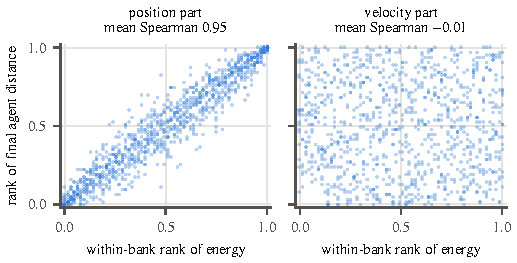
\includegraphics[width=\auditfigwidth]{fig_audit.pdf}
\caption{Within each of the \REightN{} evaluation banks (64 candidates of the released JEPA-WM planner), rank of the
position part (left) and of the velocity part (right) of the proprioceptive goal term against the rank of the true
final agent distance. The velocity part has near-zero mean within-bank rank correlation with the final agent distance;
this does not imply statistical independence or absence of information (post hoc, descriptive).}
\label{fig:audit}
\end{figure}

\paragraph{Measurements} On the 64-plan evaluation banks of the \REightN{} evaluation goals (post hoc, descriptive;
numerical identity error below $10^{-14}$):
\begin{itemize}[leftmargin=*,itemsep=1pt]
\item mean over banks of each part's within-bank mean divided by the within-bank mean of $\Pi$: position \DecJPos,
  velocity \DecJVel, cross term \DecJCross, residual and token variation together \DecJResTok;
\item mean within-bank Spearman correlation with the true final agent distance: \DecJSpFull{} for $\Pi$, \DecJSpPos{}
  for the position part and \DecJSpVel{} for the velocity part.
\end{itemize}
Velocity mismatch is thus a large part of this proprioceptive term, with near-zero \emph{average} monotone association
with the agent distance (Fig.~\ref{fig:audit}). Bank-level correlations range from \DecJSpVelMin{} to \DecJSpVelMax{};
a near-zero average neither establishes independence nor concerns every component of the success criterion. Pooling
the energies of all banks gives a velocity share of \DecJVelPooled{}, distinct from the equal-bank average of
\DecJVel. On the development banks, the predicted and encoded-true values of $\Pi$ have within-bank rank correlation
\DevSpPredTrue: the ranking problem is already present when the term is evaluated on true endpoints. This does not
show that physical prediction errors are small.

\paragraph{Conditioning} Both stored encoder matrices have full column rank. Keeping the position part is the map $h\mapsto Ah$ with $A=W_p\,[I\;0]\,W^{+}$, an
\emph{oblique} projector onto the range of $W_p$ along the range of $W_v$ and the orthogonal complement of the range of
$W$. Its operator norm is $1/\sin\theta$, where $\theta$ is the smallest principal angle between the ranges of $W_p$ and
$W_v$, a classical fact about oblique projectors \cite{simoncini2010oblique}. For JEPA-WM, $\theta=\AngJ^\circ$ and $\|A\|=\GainJ$ (condition number of $W$: \CondJ), so the
decomposition is numerically benign. Section~\ref{sec:r10} shows that this is not so for DINO-WM.

\section{The repair}
\label{sec:method}
VELDROP-z scores a candidate by
\begin{equation}
s=z(L_{\mathrm{vis}})+z(\Pi_{\mathrm{pos}}),\qquad \Pi_{\mathrm{pos}}=\|u\|^2/m,
\end{equation}
where $z(x)=(x-\bar x)/(\operatorname{sd}(x)+10^{-12})$ uses the population standard deviation over the current
candidate set. It uses no outcome labels at inference. It retains only the position energy of Eq.~\eqref{eq:decomp},
so it removes the cross, residual and token-variation terms as well as the pure velocity term. Because $AW_v=0$, the
score is invariant to a velocity-only change of the goal embedding when the predicted tokens and the visual goal are
held fixed; this algebraic invariance is not by itself a claim of better control. Its only inputs beyond the official
cost are the model's proprioceptive encoder and a declared goal-coordinate schema (which entries of $r$ are
velocities).

I selected the rule and its weighting on the development starts, where VELDROP-z gave \DevVZ{} with \DevVZSucc{}
successes against \DevOff{} and \DevOffSucc{} for the official cost; these are design-set results, not independent estimates of performance.
Development ablations also showed that dropping velocity at the official weight changes almost nothing (\DevVOne{} against \DevOff), that
standardising the full term loses successes (\DevHstdSucc{} against \DevOffSucc), and that replacing the goal velocity
by zero is worse than dropping it (\DevVzero, \DevVzeroSucc{} successes). The evaluations below keep the rule fixed, although earlier results informed its design. They also evaluate the
frozen supervised head of an earlier development round, a ridge-regression score over the 384 visual channel energies
and the proprioceptive energy fitted to development margins; it is not retrained here.

\section{Results}
\label{sec:results}

\subsection{Fixed candidate banks on evaluation goals}
\label{sec:r8}
The primary hypothesis of this locked test was the frozen supervised head against the official cost; VELDROP-z and a
mechanism check were added as a separate locked hypothesis (Appendix~\ref{app:locks}). Table~\ref{tab:r8} gives the
results on \REightN{} evaluation goals.

\begin{table}[t]
\centering
\caption{Fixed-bank selection on \REightN{} evaluation goals (64-plan banks): mean selected margin (lower is better)
with bootstrap interval, and successes.}
\label{tab:r8}
\footnotesize
\begin{tabular}{lcc}
\toprule
Selection rule & margin [95\% CI] & succ. \\
\midrule
official cost & \REightBzero{} [\REightBzeroLo, \REightBzeroHi] & \REightBzeroSucc \\
\textbf{VELDROP-z} & \textbf{\REightVZ{}} [\REightVZLo, \REightVZHi] & \textbf{\REightVZSucc} \\
supervised head (frozen) & \REightBone & \REightBoneSucc \\
proprio weight 10 (not 0.1) & \REightHten & \REightHtenSucc \\
standardised full proprio term & \REightHstd & \REightHstdSucc \\
position term only & \REightPosOnly & \REightPosOnlySucc \\
velocity dropped at weight 0.1 & \REightVOne & \REightVOneSucc \\
official cost, true endpoints & \REightEBzero & \REightEBzeroSucc \\
best plan in bank & \REightOracle & \REightOracleSucc \\
\bottomrule
\end{tabular}
\end{table}

\begin{itemize}[leftmargin=*,itemsep=1pt]
\item \emph{VELDROP-z improves fixed-bank selection.} $D=\REightVZD$ [\REightVZDLo, \REightVZDHi]; \REightVZImp{} starts improved,
  \REightVZWor{} worsened; without the most favourable start the mean is \REightVZDexcl. Successes went from
  \REightBzeroSucc{} to \REightVZSucc{} (\REightVZGain{} gained, \REightVZLoss{} lost; McNemar $p=\McNREight$), which equals
  the number of banks that contain a success: no reranking of these banks can do better on successes.
\item \emph{The position term ranks agent distance more accurately.} The position part's Spearman correlation with the agent distance
  (\REightSpPos) exceeds the full term's (\REightSpProp).
\item \emph{The frozen supervised head does not improve selection} ($D=\REightBoneD$; successes \REightBzeroSucc{} to \REightBoneSucc).
\end{itemize}

\paragraph{Fixed-bank ablations (post hoc)} Crossing the proprioceptive quantity (full or position)
with the weight rule (fixed 0.1 or standardised) on the same banks gives margins (successes): full at 0.1, \FacRaCzz{}
(\FacRaCzzSucc); position at 0.1, \FacRaCoz{} (\FacRaCozSucc); full standardised, \FacRaCzo{} (\FacRaCzoSucc); position
standardised, \FacRaCoo{} (\FacRaCooSucc). Neither change alone meets the operational improvement rule on these banks; their combination does. Position against
full under standardisation: $D=\FacRaDropD$, successes \FacRaDropGain{} gained and \FacRaDropLoss{} lost (McNemar $p=\FacRaDropMcN$). Using the standardisation scale of the full term for the position term gives \FacRaSA{}
(\FacRaSASucc), so in the banks the gain does not come from a different scale alone. Selecting by the visual term
alone gives \RaVisOnly{} (\RaVisOnlySucc) and picks the same plan as the official cost in \RaVisOnlySame{} of
\RaVisOnlyN{} banks. These contrasts were computed after the outcomes were known.

\subsection{Inside the search}
\label{sec:r9}
I locked a second test on the same goals: CEM optimises VELDROP-z (or the frozen head) with the seeds of the
official-cost CEM, and the final mean is executed. The official-cost arm is the collection's own CEM, reproduced
bit-exactly by a rerun on the first start. Table~\ref{tab:r9} gives the results.

\begin{widetable}[t]
\centering
\caption{The score used as the CEM objective, \RNineN{} goals (same goals as Table~\ref{tab:r8}); final CEM mean
executed open loop. Mean executed margin with bootstrap interval, successes, block-only successes and mean errors.}
\label{tab:r9}
\small
\begin{tabular}{lccccc}
\toprule
CEM objective & margin [95\% CI] & succ. & block only & agent err. & block err. \\
\midrule
official cost & \RNineBzeroMargin{} [\RNineBzeroMarginLo, \RNineBzeroMarginHi] & \RNineBzeroSucc & \RNineBzeroBlockOnly & \RNineBzeroAgent & \RNineBzeroBlock \\
\textbf{VELDROP-z} & \textbf{\RNineVZMargin{}} [\RNineVZMarginLo, \RNineVZMarginHi] & \textbf{\RNineVZSucc} & \RNineVZBlockOnly & \RNineVZAgent & \RNineVZBlock \\
supervised head (frozen) & \RNineBoneMargin{} [\RNineBoneMarginLo, \RNineBoneMarginHi] & \RNineBoneSucc & \RNineBoneBlockOnly & \RNineBoneAgent & \RNineBoneBlock \\
\bottomrule
\end{tabular}
\end{widetable}

\begin{itemize}[leftmargin=*,itemsep=1pt]
\item \emph{VELDROP-z lowers executed margin inside CEM.} $D=\RNineVZD$ [\RNineVZDLo, \RNineVZDHi]; \RNineVZImp{} starts improved and
  \RNineVZWor{} worsened (sign test $p=\SignRNine$); without the most favourable start \RNineVZDexcl. Successes
  \RNineBzeroSucc{} to \RNineVZSucc, with \RNineVZGain{} gained and \RNineVZLoss{} lost (McNemar $p=\McNRNine$): the success-count difference is uncertain at this sample size. The largest reduction of position
  error is for the agent (\RNineBzeroAgent{} to \RNineVZAgent; block-only successes unchanged). This is consistent with
  the proposed explanation but does not isolate its causal contribution.
\item \emph{The supervised head degrades in-search performance.} $D=\RNineBoneD$; successes \RNineBzeroSucc{} to \RNineBoneSucc{}
  (\RNineBoneGainN{} gained, \RNineBoneLossN{} lost). Its executed plan scored \emph{worse under the head itself} than
  the official-cost plan on \BoneOwnWorse{} of \BoneOwnN{} starts (mean predicted head score \BoneOwnBone{} versus
  \BoneOwnBzero), so the search did not reliably improve even its own objective; this alone does not explain the
  lost successes.
\end{itemize}

\paragraph{Retained component and weighting inside CEM} VELDROP-z changes two things at
once: it keeps only the position part, and it replaces the fixed weight 0.1 by standardisation within each
population. I therefore ran the two missing cells of the $2\times2$ design on the same goals and seeds, under a
protocol locked before these runs: the full term standardised, $z(L_{\mathrm{vis}})+z(\Pi)$, and the position part at
the official weight, $L_{\mathrm{vis}}+0.1\,\Pi_{\mathrm{pos}}$. A rerun of the official-cost search on the first start
again reproduced the stored plan bit-exactly. Table~\ref{tab:r11} gives the four cells.

\begin{table}[t]
\centering
\caption{The $2\times2$ factorial inside CEM on the \RElN{} goals of Table~\ref{tab:r9}: mean executed margin (lower is
better), successes and mean final agent error. The full term and the position part at weight 0.1 versus standardised
within each population.}
\label{tab:r11}
\footnotesize
\begin{tabular}{lccc}
\toprule
proprio quantity, weight & margin & succ. & agent err. \\
\midrule
full, 0.1 (official) & \RElCzz & \RElCzzSucc & \RElCzzAgent \\
position, 0.1 & \RElCoz & \RElCozSucc & \RElCozAgent \\
full, standardised & \RElCzo & \RElCzoSucc & \RElCzoAgent \\
position, standardised (VELDROP-z) & \RElCoo & \RElCooSucc & \RElCooAgent \\
\bottomrule
\end{tabular}
\end{table}

\begin{itemize}[leftmargin=*,itemsep=1pt]
\item \emph{Standardising the full term gives the larger contrast on this cohort.} It lowered the executed margin by
  \RElScaleFull{} [\RElScaleFullLo, \RElScaleFullHi] relative to the official cost (\RElScaleFullImp{} starts improved,
  \RElScaleFullWor{} worsened) but left successes unchanged (\RElScaleFullGain{} gained, \RElScaleFullLoss{} lost).
  Within each population its ranking is that of $L_{\mathrm{vis}}+\alpha_t\Pi$ with
  $\alpha_t=(\operatorname{sd}(L_{\mathrm{vis}})+10^{-12})/(\operatorname{sd}(\Pi)+10^{-12})$. Across the \RElNPop{}
  search populations of this arm, $\alpha_t$ averages \RElAlphaFull{} (from \RElAlphaFullMin{} to \RElAlphaFullMax),
  about \RElEffFold{} times the official 0.1 on average; it is not a fixed weight.
\item \emph{The standardised position-only rule has \RElGain{} more successes than the standardised full rule.} In the
  pre-specified primary contrast, the position part against the full term under standardisation
  gave $D=\RElD$ [\RElDLo, \RElDHi] (median \RElMedian; \RElImp{} improved, \RElWor{} worsened; without the most
  favourable start \RElDexcl) and \RElGain{} additional successes with \RElLoss{} lost (McNemar $p=\RElMcN$). The operational
  rule is met, but the interval reaches zero and the success difference is not significant, so this is weak evidence.
  The contrast changes both the retained component and its own standardisation denominator; it is not an intervention
  on velocity at a fixed numerical weight.
\item \emph{At the official weight, the position-only contrast is uncertain} ($D=\RElSecD$ [\RElSecDLo,
  \RElSecDHi]; successes \RElSecGain{} gained, \RElSecLoss{} lost), as in the fixed banks. This is consistent with the
  scales logged in this arm: at weight 0.1, the position term's standard deviation within a search population is on
  average \RElVOnePosRatio{} times smaller than the visual term's, and at least \RElVOnePosRatioMin{} times smaller in
  every population. Interaction \RElInter{} [\RElInterLo, \RElInterHi].
\end{itemize}
The two paths through Table~\ref{tab:r11} split the total change of \RNineVZD{} differently (\RElScaleFull{} then
\RElD, or \RElSecD{} then \RElScalePos), and on both paths the four extra successes appear only in the last step, so
neither path allocates the gain to one ingredient. Section~\ref{sec:r12} adds a comparison at a frozen weight on a fresh
cohort. Fixed banks and in-search runs also differ in kind: one selects among the raw planner's candidates, the other
changes the candidates and executes an elite mean, so their outcomes need not agree.

\subsection{A fresh cohort}
\label{sec:r12}
To repeat the in-search tests on goals that played no earlier role, I locked a test on \RTwN{} new starts. Each start
runs CEM arms with the same seed, so all arms share the first population $Q_0$: the official cost, VELDROP-z,
$L_{\mathrm{vis}}+\alpha_0\Pi$ and $L_{\mathrm{vis}}+\alpha_0\Pi_{\mathrm{pos}}$. Here $\alpha_0=(\operatorname{sd}(L_{\mathrm{vis}})+10^{-12})/
(\operatorname{sd}(\Pi)+10^{-12})$ is computed once on $Q_0$ and frozen for all iterations; it averages
\RTwAlphaMean{} (from \RTwAlphaMin{} to \RTwAlphaMax), about \RTwAlphaFold{} times the official 0.1. The primary question
was the frozen-weight comparison of the two terms; VELDROP-z against the official cost was a pre-declared secondary
question. After these four arms had been analysed, a fifth arm, the standardised full term $z(L_{\mathrm{vis}})+z(\Pi)$,
was locked and run on the same starts to repeat the primary contrast of Table~\ref{tab:r11}. Table~\ref{tab:r12} gives
all five arms.

\begin{table}[t]
\centering
\caption{Fresh cohort of \RTwN{} starts; the score is the CEM objective and the final mean is executed open loop. Mean
executed margin, successes, block-only successes, and mean agent and block errors.}
\label{tab:r12}
\footnotesize
\setlength{\tabcolsep}{4pt}
\begin{tabular}{lccccc}
\toprule
CEM objective & margin & succ. & block only & agent & block \\
\midrule
official cost & \RTwRawMargin & \RTwRawSucc & \RTwRawBO & \RTwRawAgent & \RTwRawBlock \\
full, frozen $\alpha_0$ & \RTwFFMargin & \RTwFFSucc & \RTwFFBO & \RTwFFAgent & \RTwFFBlock \\
position, frozen $\alpha_0$ & \RTwFPMargin & \RTwFPSucc & \RTwFPBO & \RTwFPAgent & \RTwFPBlock \\
full, standardised & \RThMargin & \RThSucc & \RThBO & \RThAgent & \RThBlock \\
\textbf{VELDROP-z} & \textbf{\RTwVZMargin} & \textbf{\RTwVZSucc} & \RTwVZBO & \RTwVZAgent & \RTwVZBlock \\
\bottomrule
\end{tabular}
\end{table}

\begin{figure}[t]
\centering
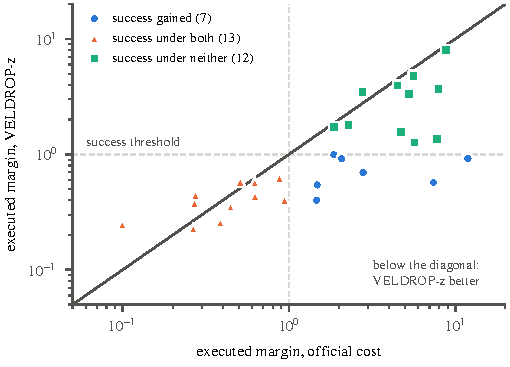
\includegraphics[width=\columnwidth]{fig_fresh.pdf}
\caption{Fresh cohort of \RTwN{} starts: executed margin of the final CEM plan under the official cost and under
VELDROP-z (log scales; one point per start). Points below the diagonal improved; the dashed lines mark the success
threshold. \RTwQTwoGain{} starts gained a success and none lost one.}
\label{fig:fresh}
\end{figure}

\begin{itemize}[leftmargin=*,itemsep=1pt]
\item \emph{VELDROP-z against the official cost (pre-specified secondary).} $D=\RTwQTwoD$ [\RTwQTwoLo, \RTwQTwoHi]
  (median \RTwQTwoMed; \RTwQTwoImp{} starts improved, \RTwQTwoWor{} worsened; sign test $p=\RTwQTwoSign$; without the most
  favourable start \RTwQTwoLBO). Successes rose from \RTwRawSucc{} to \RTwVZSucc, with \RTwQTwoGain{} gained and
  \RTwQTwoLoss{} lost (exact McNemar $p=\RTwQTwoMcN$; Fig.~\ref{fig:fresh}). This repeats the earlier in-search
  result on fresh goals. The largest mean error reduction is
  again for agent placement (agent error \RTwRawAgent{} to \RTwVZAgent), while the mean block error rose from
  \RTwRawBlock{} to \RTwVZBlock.
\item \emph{Position against full at the frozen weight (primary).} $D=\RTwQOneD$ [\RTwQOneLo,
  \RTwQOneHi] (median \RTwQOneMed; \RTwQOneImp{} improved, \RTwQOneWor{} worsened; sign test $p=\RTwQOneSign$; without the
  most favourable start \RTwQOneLBO), with \RTwQOneGain{} success gained and \RTwQOneLoss{} lost. The operational rule is
  met, but the interval contains zero. The point estimate favours the position term; the interval also permits a
  larger gain or a slight degradation. This is not an equivalence test. The contrast removes the cross, residual and token-variation terms together with the velocity term.
\item \emph{Descriptive contrasts.} Both frozen-weight rules improve on the official cost (full \RTwFFRawD{}
  [\RTwFFRawLo, \RTwFFRawHi], position \RTwFPRawD{} [\RTwFPRawLo, \RTwFPRawHi]), with one net success each. VELDROP-z
  improves on the frozen-weight position rule by \RTwVZFPD{} [\RTwVZFPLo, \RTwVZFPHi], with \RTwVZFPGain{} successes
  gained and \RTwVZFPLoss{} lost.
\item \emph{Position against full under standardisation (exploratory added arm).} $D=\RThD$ [\RThLo, \RThHi] (median
  \RThMed; \RThImp{} improved, \RThWor{} worsened; sign test $p=\RThSign$; without the most favourable start \RThLBO), with
  \RThGain{} successes gained and \RThLoss{} lost (exact McNemar $p=\RThMcN$). Standardising the full term itself changes the
  margin by \RThStdRawD{} [\RThStdRawLo, \RThStdRawHi] relative to the official cost, with \RThStdRawGain{} successes
  gained and \RThStdRawLoss{} lost. Of the \RTwQTwoGain{} starts that VELDROP-z adds over the official cost, two are
  already successes under the standardised full term.
\end{itemize}
The fresh cohort thus repeats the pattern of Table~\ref{tab:r11}. The step from the official cost to the standardised
full term is the larger margin change (\RThStdRawD), and the further switch to the position term comes with the success
gains (\RThGain{} gained, \RThLoss{} lost) but an uncertain margin difference; at the frozen intermediate weight the
contrast remains uncertain. The weight that VELDROP-z implicitly gives the position term,
$(\operatorname{sd}(L_{\mathrm{vis}})+10^{-12})/(\operatorname{sd}(\Pi_{\mathrm{pos}})+10^{-12})$, has a median of \RTwVZWFirst{} in the
first population and \RTwVZWLast{} in the last (post hoc), while $\alpha_0$ stays fixed. One untested reading is that
the velocity-related terms matter mainly when proprioception carries a large weight.

\subsection{A second released model}
\label{sec:r10}
DINO-WM uses the same frozen DINOv2 encoder, its own predictor, a $\mathrm{Linear}(4\to20)$ proprioceptive encoder, and
a goal cost of the same form. I locked an unchanged \mbox{VELDROP-z} test on \RTenN{} new training-split goals (fixed banks).
\begin{itemize}[leftmargin=*,itemsep=1pt]
\item \emph{Selection improves slightly, with unchanged successes.} \RTenVZ{} against \RTenBzero{} ($D=\RTenVZD$; \RTenVZImp{} improved,
  \RTenVZWor{} worsened, \RTenUnchanged{} unchanged; sign test $p=\SignRTen$). With five zero differences, a bootstrap
  resample consists only of zeros with probability \BootZeroRTen, so the percentile interval is not strong evidence.
  The official cost and both standardised rules attain the same \RTenBzeroSucc{} successful banks.
\item \emph{Velocity mismatch is small in DINO-WM.} Velocity carries \DecDnVel{} of the proprioceptive term (position
  \DecDnPos), and the full term already ranks candidates by the agent distance (Spearman \DecDnSpFull).
\end{itemize}
DINO-WM's encoder is much less sensitive to velocity in normalised coordinates: its velocity columns have norms
\EncDinoVx{} and \EncDinoVy, against \EncDinoX{} and \EncDinoY{} for position. They are also nearly parallel to the
position columns ($\theta=\AngDn^\circ$, condition number \CondDn), so the position-only map amplifies embedding errors
up to $\|A\|=\GainDn$ times. On these banks VELDROP-z selected the same plan as the standardised full term on
\SameSelDino{} of \SameSelDinoN{} starts: re-weighting the full term reproduces the observed selections, so these banks
show no incremental selection benefit from dropping the velocity-related terms. Because the stored predictions are
rounded to 16 bits, I re-scored every DINO-WM evaluation bank in 32 bits, with four JEPA-WM banks as a control: the
stored costs and tokens were reproduced exactly, no selection changed (\FpDnN{} DINO-WM and \FpJN{} JEPA-WM banks), and
the largest relative change of the position energy was \FpDnMaxRel{} (DINO-WM) and \FpJMaxRel{} (JEPA-WM). The
DINO-WM projection nevertheless remains poorly conditioned for perturbations in other directions.

\section{Negative results}
\label{sec:negative}
The frozen supervised scoring head had shown a favourable transfer estimate in earlier development, yet it produced \REightBoneSucc{} successes in the JEPA-WM fixed banks against \REightBzeroSucc{} for the
official cost, and \RNineBoneSucc{} against \RNineBzeroSucc{} inside CEM. Increasing the full proprioceptive weight
from 0.1 to 10 (100-fold), or standardising the full term, lowered the mean margin but lost successes in fixed banks
(Table~\ref{tab:r8}); inside CEM, standardising the full term lowered the margin while keeping the success count at
\RElCzoSucc{} (\RElScaleFullGain{} gain, \RElScaleFullLoss{} loss). Aggregate rank correlations and fixed-bank outcomes
therefore cannot substitute for evaluating a cost inside the search. Two training-free visual energies from earlier
rounds also failed their own locked tests: an optimal-transport patch energy was refuted by its mechanism probe, and
tail pooling of patch errors gave $D=\RSevenTpeD$ [\RSevenTpeDLo, \RSevenTpeDHi]. I report these failures alongside the
positive rule.

\section{Limitations}
\begin{itemize}[leftmargin=*,itemsep=1pt]
\item \emph{Scope.} One task; two released checkpoints; CEM at $64\times8$ rather than $300\times30$; one open-loop plan
  rather than receding-horizon control.
\item \emph{Dependence and statistics.} The fixed-bank, in-search and factorial tests use the same \REightN{} goals and
  are not independent replications; the fresh cohort of \RTwN{} starts is the only repetition on new goals, and the
  DINO-WM test is a fixed-bank test. Small cohorts and skewed paired differences can make percentile-bootstrap coverage unreliable. Several decisions were pre-specified across rounds and earlier development rounds
  chose the direction, so the results are not corrected for multiplicity. On the fresh cohort, two questions were
  pre-declared and a third was added after their analysis; the success differences there have exact McNemar values of
  \RTwQTwoMcN{} (VELDROP-z against the official cost) and \RThMcN{} (position against full under standardisation),
  uncorrected. Descriptive comparisons of VELDROP-z with either frozen-weight arm also have nominal McNemar $p=0.0312$ (six gains, no losses); these do not provide multiplicity-controlled confirmation.
\item \emph{Data.} All evaluation goals, the fresh cohort included, come from training-split trajectories of the
  checkpoints.
\item \emph{Mechanism scope.} The mechanism needs a goal whose proprioception contains a velocity the criterion ignores
  and an encoder that is sensitive to it. The velocity energy is large in the JEPA-WM banks and small in the DINO-WM
  banks; other tasks are untested.
\item \emph{Design.} The equal weighting of the two standardised terms is a heuristic. In development, weights from
  \DevSensLamMin{} to \DevSensLamMax{} on the standardised position term gave mean margins from \DevSensMinMean{} to
  \DevSensMaxMean{} with \DevSensSuccMin{} to \DevSensSuccMax{} successes, against \DevOff{} and \DevOffSucc{} for the
  official cost; smaller weights gave smaller gains. The goal-coordinate schema is task knowledge.
\end{itemize}

\section{Conclusion}
The released JEPA-WM PushT cost penalises a goal-frame velocity that its endpoint success criterion does not require.
An exact decomposition shows that this velocity carries most of the proprioceptive goal energy and has a
near-zero mean within-bank rank correlation with the final agent distance, while at the official weight of 0.1 the visual term alone selects the same plan in \RaVisOnlySame{} of \RaVisOnlyN{} fixed banks. Keeping the decoded position energy and standardising it against the visual term
(VELDROP-z) improved the executed plans of reduced-budget search, first on \RNineN{} goals and then on a fresh cohort of
\RTwN{} starts, where successes rose from \RTwRawSucc{} to \RTwVZSucc{} with no losses. Standardising the full term
instead also lowered the margin, but its success counts went from \REightBzeroSucc{} to \REightHstdSucc, from
\RElCzzSucc{} to \RElCzoSucc{} and from \RTwRawSucc{} to \RThSucc{} across the three evaluations. Inside the search, the
direct comparisons of the two terms under standardisation gave \RElGain{} and \RThGain{} success gains with no losses, but
margin intervals that include zero, and at a frozen intermediate weight the difference remained uncertain. These comparisons do not isolate a
pure-velocity effect or allocate the total gain. DINO-WM, whose encoder is far less sensitive to velocity, is a boundary
case with no incremental benefit over standardised full proprioception. For planners with a full-column-rank linear proprioceptive encoder, the same decomposition applies. More generally, the audit suggests a procedure: decompose the goal term by what the goal encodes, compare each part with what the success
criterion depends on, and test a repair inside the search rather than only on fixed candidates. Release-budget
receding-horizon control, several seeds per start, goals outside the training split and other tasks are needed before
broader claims.

\appendices
\section{Locks, timestamps and deviations}
\label{app:locks}
\begin{itemize}[leftmargin=*,itemsep=1pt]
\item \emph{Fixed-bank test.} Locked at 02:32 UTC on 27 Oct 2026 before any data. The VELDROP-z addendum, the mechanism
  check and the in-search protocol were locked at 02:52, when 3 of 16 starts had been collected; according to the
  execution log, none had been opened.
\item \emph{DINO-WM test.} Locked at 04:58 and amended at 05:00 to a fixed eight-start cohort, before any data.
\item \emph{Factorial inside the search.} Designed after the earlier outcomes were known, and recorded at 23:48 UTC on
  27 Oct 2026 (06:48 on 28 Oct, Vietnam time) before its runs; it is development evidence on the same goals.
\item \emph{Fresh cohort.} Locked at 07:54 UTC on 28 Oct 2026, after infrastructure checks on an old start (the
  official-cost search reproduced its stored plan exactly) and before any run of the cohort. It ran in nine resumable
  chunks whose logs print timing and $\alpha_0$ only, and it was analysed once, after all 128 runs, then re-checked by a
  second implementation. No run crashed.
\item \emph{Standardised full arm on the fresh cohort.} Added after the analysis of the first four arms and locked at
  23:41 UTC on 28 Oct 2026 before its runs. A restart of the computing container stopped its collection after four
  runs; the interrupted run was repeated from its seed with unchanged code, and the interruption is recorded in the
  deviation log. It was analysed once and re-checked by a second implementation.
\item \emph{Execution deviations.} The first in-search test ran in three resumable chunks; one console log was
  overwritten and another stayed empty (each run record keeps its own timing), and two run records were printed during a
  format check before the analysis. A first DINO-WM launch, started concurrently against its lock, was killed before it
  recorded any start.
\item \emph{Post hoc material.} The five-part decomposition shares, the bank factorial, the encoder geometry, the
  agreement between VELDROP-z and the standardised full term on DINO-WM, and the head's own-score comparison were
  computed after the outcomes and are descriptive.
\item \emph{Verification.} Separate analysis implementations reproduced the recorded numerical decisions from saved per-plan
  components and terminal states. The fresh-cohort audit additionally checks all 160 terminal records, five-arm goal
  and initial-population matching, and constancy of the frozen weights. This verifies the saved-result
  analysis, not an independent repetition of model training or of all simulator collection. The accompanying artifact provides portable saved-result analyses and external-runtime collection
  scripts. A complete collection rerun requires the released checkpoints, datasets and pinned upstream repositories;
  those dependencies are not bundled. The analysis code, run records and manuscript sources are available at
  \url{https://github.com/levanmanh268/jepa-goal-cost-audit}.
\end{itemize}


\begin{thebibliography}{99}\small
\bibitem{zhou2024dinowm} G.~Zhou, H.~Pan, Y.~LeCun, L.~Pinto. DINO-WM: World models on pre-trained visual features enable zero-shot planning. arXiv:2411.04983, 2024.
\bibitem{terver2025jepawm} B.~Terver, T.-Y.~Yang, J.~Ponce, A.~Bardes, Y.~LeCun. What drives success in physical planning with joint-embedding predictive world models? TMLR 2026; arXiv:2512.24497.
\bibitem{maes2026lewm} L.~Maes, Q.~Le~Lidec, D.~Scieur, Y.~LeCun, R.~Balestriero. LeWorldModel: Stable end-to-end joint-embedding predictive architecture from pixels. arXiv:2603.19312, 2026.
\bibitem{chi2023diffusionpolicy} C.~Chi et al. Diffusion policy: Visuomotor policy learning via action diffusion. RSS 2023.
\bibitem{li2026trm} L.~Li, S.~Wang, L.~Qiu, M.~Xiong, Q.~Liu. World model control by trajectory reachability metrics. arXiv:2605.22164, 2026.
\bibitem{jang2026projection} Y.~S.~Jang, M.~S.~Ryoo. Latent projection for latent planning. arXiv:2610.26979, 2026.
\bibitem{pham2026leap} P.~Pham, A.~Bera. Latent energy action planning with world models. arXiv:2609.03294, 2026.
\bibitem{kang2026aniso} M.~Kang, Y.~Oh, S.~Kim, J.~Lee. Anisotropic representations improve planning in JEPA world models. arXiv:2609.37441, 2026.
\bibitem{moukheiber2026tempo} L.~Moukheiber, H.~Xue, Y.~Chen. How long, not how close: A learned temporal metric for planning in latent world models. arXiv:2610.04988, 2026.
\bibitem{you2026ngc} Z.~You, L.~Tao, S.~Xu, Y.~Wang, C.~Xu. Latent world models should plan with distances along the latent manifold. arXiv:2610.25013, 2026.
\bibitem{destrade2026value} M.~Destrade, O.~Bounou, Q.~Le~Lidec, J.~Ponce, Y.~LeCun. Value-guided action planning with JEPA world models. arXiv:2601.00844, 2026.
\bibitem{strohm2026little} F.~Strohm, P.~Wagner, J.~Schwab, M.~Huber. Keeping JEPA world models plannable when little of the frame moves. arXiv:2610.03137, 2026.
\bibitem{hara2026criterion} T.~Hara, K.~Suzuki. Supervise what decides success: Criterion-aligned auxiliary losses for latent world-model planning. arXiv:2610.01224, 2026.
\bibitem{min2026misleads} R.~Min, X.~Li, F.~Xu, E.~J.~Du. When low prediction error misleads planning: Diagnosing representation, dynamics, and decision failures in latent world models. arXiv:2610.05550, 2026.
\bibitem{wang2026dalewm} J.~Wang, Y.~Zuo, K.~Rui, Y.~Feng, M.~Li. Decision-metric alignment in latent world models: Diagnostics and action-conditioned objectives for MPC planning. arXiv:2608.18746, 2026.
\bibitem{andrychowicz2017her} M.~Andrychowicz, F.~Wolski, A.~Ray, J.~Schneider, R.~Fong, P.~Welinder, B.~McGrew, J.~Tobin, P.~Abbeel, W.~Zaremba. Hindsight experience replay. NeurIPS 2017; arXiv:1707.01495.
\bibitem{velez2026gsher} C.~V\'elez Garc\'ia, M.~Cazorla, J.~Pomares. Goal sets, not goal states: Queryable robot goals through goal-set hindsight relabeling. arXiv:2606.09476, 2026.
\bibitem{wu2026firm} Y.~Wu, Y.~Zhang, A.~Li, M.~Wang, H.~Wu, A.~Zhang. FIRM-WM: State-factorized factual-interventional recurrent modeling for reward-free visual planning. arXiv:2609.22816, 2026.
\bibitem{ebert2018foresight} F.~Ebert, C.~Finn, S.~Dasari, A.~Xie, A.~Lee, S.~Levine. Visual Foresight: Model-based deep reinforcement learning for vision-based robotic control. arXiv:1812.00568, 2018.
\bibitem{tian2020functional} S.~Tian, S.~Nair, F.~Ebert, S.~Dasari, B.~Eysenbach, C.~Finn, S.~Levine. Model-based visual planning with self-supervised functional distances. arXiv:2012.15373, 2020.
\bibitem{lambert2020mismatch} N.~Lambert, B.~Amos, O.~Yadan, R.~Calandra. Objective mismatch in model-based reinforcement learning. arXiv:2002.04523, 2020.
\bibitem{simoncini2010oblique} V.~Simoncini, D.~B.~Szyld. On the field of values of oblique projections. Linear Algebra Appl., 433:810-818, 2010.
\end{thebibliography}

\end{document}
